\chapter{Динамика Фридмана: материя, излучение и энергия вакуума}

\lectureoverview{Кинематику расширяющейся Вселенной можно выразить
одной строкой: физические расстояния растут с масштабным фактором \(a(t)\). Теперь задача
состоит в том, чтобы определить эту функцию. Мы восстановим уравнение
Фридмана для плоского пространства из ньютоновского закона сохранения
энергии, сначала решим его для обычной материи, а затем увидим, почему излучение и энергия
вакуума приводят к совершенно различным космическим историям.}

\section{Геометрия, которую предстоит объяснить}

При фиксированном космическом времени крупномасштабная Вселенная выглядит однородной и
изотропной. Галактики, скопления и сверхскопления, конечно, являются реальными структурами,
но на масштабах в сотни миллионов или миллиарды световых лет их
распределение становится поразительно равномерным. Эта эмпирическая
закономерность называется космологическим принципом. Само название не делает его
теоремой; его сила основана на наблюдениях.

Есть и второй эмпирический факт. В пределах нынешней точности большие
пространственные треугольники ведут себя как евклидовы. Сравнение с
геодезической съёмкой футбольного поля здесь полезно. Если туго натянутые
линии образуют треугольники, сумма углов которых равна \(180^\circ\), этим ещё не доказано, что Земля
глобально плоская. Показано лишь, что радиус кривизны Земли велик по сравнению
с полем. Космическая съёмка имеет ту же логическую форму: пространство может иметь очень
большой радиус кривизны, но в пределах наблюдаемой области оно хорошо
приближённо описывается как плоское.

Эталонная геометрия — пространство-время Минковского,
\begin{equation}
  d\tau^2=dt^2-\left(dx^2+dy^2+dz^2\right).
  \label{eq:l09-minkowski}
\end{equation}
Выражение в скобках — просто евклидов элемент расстояния в трёх измерениях. В
общей теории относительности, напротив, коэффициенты при координатных
дифференциалах являются полями. Они могут зависеть от положения и времени, и могут также возникать смешанные члены.
Эти метрические коэффициенты — релятивистские аналоги ньютоновского
гравитационного поля.

\begin{figure}[H]
  \centering
  \includegraphics[width=0.72\textwidth]{lecture_09_figure_01.png}
  \caption{Элемент собственного времени Минковского, записанный в начале
  лекции. Исходный кадр: 00:01:50.}
  \label{fig:l09-minkowski-board}
\end{figure}

Для пространственно плоской расширяющейся Вселенной однородность и изотропия оставляют один
зависящий от времени масштабный фактор:
\begin{equation}
  d\tau^2=dt^2-a^2(t)\left(dx^2+dy^2+dz^2\right).
  \label{eq:l09-flat-frw}
\end{equation}
Мы используем единицы, в которых \(c=1\), поэтому время и длина имеют одну и ту же размерность.
Существуют две согласованные конвенции. Можно придать \(x,y,z\) размерность
длины и считать \(a\) безразмерным, либо трактовать \(x,y,z\) как безразмерные
метки, а размерность длины отнести к \(a\). В лекции используется вторая
конвенция, потому что она делает физический смысл \(a(t)\) наглядным.

\begin{figure}[H]
  \centering
  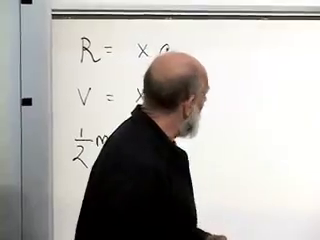
\includegraphics[width=0.72\textwidth]{lecture_09_figure_02.png}
  \caption{Плоская расширяющаяся метрика, в которой масштабный фактор умножает
  евклидов пространственный элемент длины. Исходный кадр: 00:09:12.}
  \label{fig:l09-expanding-metric-board}
\end{figure}

Представьте себе координаты, нанесённые на резиновый лист. Координатные метки остаются
прикреплёнными к листу, тогда как физическое расстояние между ними растёт. Поэтому такая
разность координат, как «от \(x=0\) до \(x=1\)», — это лишь пара меток. Расстояние,
представляемое этим интервалом, равно \(a(t)\). Найти уравнение, управляющее этим
масштабным фактором, — и есть динамическая задача лекции.

\section{Замкнутая, плоская и открытая пространственные геометрии}

Плоскостность — это наблюдательное упрощение, а не следствие
однородности. Существуют три однородные и изотропные пространственные геометрии:
с положительной, нулевой и отрицательной кривизной. Чтобы понять случай
положительной кривизны, полезно быть точным в отношении размерности.

Геометрическое место точек
\begin{equation}
  X_1^2+X_2^2=R^2
\end{equation}
есть окружность, или одномерная сфера \(S^1\). Её заполненная внутренняя область — это диск, который также называют
двумерным шаром. Добавление ещё одной координаты вложения даёт
\begin{equation}
  X_1^2+X_2^2+X_3^2=R^2,
\end{equation}
обычную двумерную сферу \(S^2\). Добавление четвёртой координаты вложения даёт
\begin{equation}
  X_1^2+X_2^2+X_3^2+X_4^2=R^2,
  \label{eq:l09-three-sphere}
\end{equation}
трёхсферу \(S^3\), которая сама является трёхмерным пространством. Мы не можем
наглядно представить её четырёхмерное вложение, но внутренняя геометрия не нуждается
в таком вложении, чтобы существовать.

\begin{figure}[H]
  \centering
  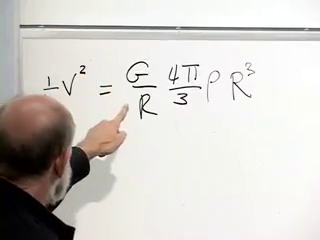
\includegraphics[width=0.72\textwidth]{lecture_09_figure_03.png}
  \caption{Уравнение вложения, используемое для введения трёхсферы. Исходный
  кадр: 00:16:40.}
  \label{fig:l09-three-sphere-board}
\end{figure}

Каждая точка идеальной сферы геометрически эквивалентна любой другой,
и любое направление в точке эквивалентно любому другому. Поэтому сфера и
однородна, и изотропна. Если её радиус умножить на \(a(t)\), всё
пространство расширяется или сжимается, не выделяя никакого центра на самой сфере. Прослеживание
такой Вселенной назад во времени не помещает всю материю в одно особое место
во внешней пустоте. Малым становится всё пространство, поэтому любая пара точек
оказывается близкой. Большой взрыв — не взрыв из одной точки пространства.

На сфере положительной кривизны сумма углов геодезических треугольников больше
\(180^\circ\). У плоских треугольников сумма углов в точности равна \(180^\circ\). В
однородной геометрии отрицательной кривизны, лишь приблизительно изображаемой седлом,
сумма углов меньше \(180^\circ\). Эти внутренние критерии различают
три случая.

\begin{figure}[H]
  \centering
  \includegraphics[width=0.72\textwidth]{lecture_09_figure_07.png}
  \caption{Положительная, нулевая и отрицательная кривизна, схематически показанные через их
  характерные формы треугольников. Исходный кадр: 00:37:30.}
  \label{fig:l09-curvature-board}
\end{figure}

Совершенно плоская локальная метрика сама по себе не доказывает, что пространство
топологически бесконечно. Компактные плоские топологии математически возможны,
хотя в лекции принимается простейшая бесконечная евклидова модель.
\editorialnote{Эта оговорка о глобальной топологии не требуется для всей
последующей локальной динамики.}

\section{Сопутствующие метки и закон Хаббла}

Теперь вернёмся к расширяющемуся плоскому листу и нанесём на него координатную сетку. В
сопутствующих координатах сетка расширяется вместе с крупномасштабным потоком материи. Галактика,
или, точнее, достаточно грубо усреднённое скопление галактик,
сохраняет приблизительно фиксированную координатную метку, хотя её физическое
расстояние до другого сопутствующего объекта меняется.

\begin{figure}[H]
  \centering
  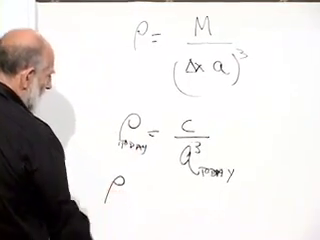
\includegraphics[width=0.72\textwidth]{lecture_09_figure_04.png}
  \caption{Координатная сетка, увлекаемая расширяющимся пространственным листом.
  Исходный кадр: 00:22:20.}
  \label{fig:l09-comoving-grid-board}
\end{figure}

Для двух объектов, разделённых вдоль оси \(x\) фиксированным сопутствующим интервалом
\(\Delta x\), физическое расстояние между ними равно
\begin{equation}
  D(t)=a(t)\,\Delta x.
  \label{eq:l09-physical-distance}
\end{equation}
Дифференцируя при фиксированном \(\Delta x\), получаем
\begin{equation}
  v(t)=\dot a(t)\,\Delta x
      =\frac{\dot a(t)}{a(t)}D(t).
\end{equation}
Введя определение
\begin{equation}
  H(t)\equiv\frac{\dot a(t)}{a(t)},
  \label{eq:l09-hubble-parameter}
\end{equation}
получаем закон Хаббла,
\begin{equation}
  v=H(t)D.
  \label{eq:l09-hubble-law}
\end{equation}
Слово «постоянная» в выражении «постоянная Хаббла» означает постоянство в
пространстве при заданном космическом времени. Оно не подразумевает постоянства
на протяжении космической истории.

\begin{figure}[H]
  \centering
  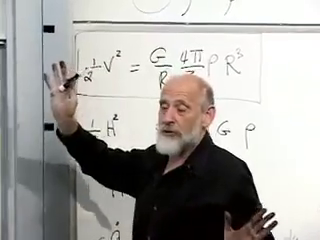
\includegraphics[width=0.72\textwidth]{lecture_09_figure_05.png}
  \caption{Вывод на доске: \(D=a\Delta x\),
  \(v=(\dot a/a)D=HD\). Исходный кадр: 00:26:40.}
  \label{fig:l09-hubble-board}
\end{figure}

\begin{classroomqa}
\audiencequestion{Если далёкая галактика наблюдается в более ранний момент
времени, должен ли выведенный для неё параметр Хаббла действительно совпадать со
значением, измеренным сегодня поблизости?}
\lecturerresponse{Только когда время, на которое мы заглядываем в прошлое,
мало по сравнению с возрастом Вселенной. На умеренных расстояниях \(H(t)\) меняется настолько
мало, что полезно пользоваться одним числом. На по-настоящему космологических расстояниях мы видим
более ранние эпохи, и зависимость \(a\) и \(H\) от времени необходимо учитывать. Это одна из причин, по которым нам
нужно динамическое уравнение для масштабного фактора.}
\end{classroomqa}

\section{Нулевые лучи в расширяющейся системе координат}

\begin{classroomqa}
\audiencequestion{Влияет ли масштабный фактор на распространение света
между далёкими галактиками?}
\lecturerresponse{Световой луч идёт по нулевой траектории, поэтому \(d\tau=0\). Для
луча, движущегося вдоль положительного направления оси \(x\), \(dy=dz=0\), и расширяющаяся метрика
даёт
\begin{align}
  0&=dt^2-a^2(t)dx^2,
  &dt&=a(t)dx,\notag\\
  &&\frac{dx}{dt}&=\frac{1}{a(t)}.
  \label{eq:l09-null-ray}
\end{align}
Координатная скорость убывает по мере роста \(a(t)\), однако локальная физическая скорость
света остаётся \(c=1\). Фиксированный координатный интервал соответствует
увеличивающемуся физическому расстоянию.}
\end{classroomqa}

\begin{figure}[H]
  \centering
  \includegraphics[width=0.72\textwidth]{lecture_09_figure_06.png}
  \caption{Нулевое условие и \(dt=a(t)dx\) для радиального распространения света.
  Исходный кадр: 00:30:54.}
  \label{fig:l09-null-board}
\end{figure}

Можно выбрать координаты, в которых тот же факт формулируется как «свет замедляется
вдали», но тогда длины и часы приходится описывать столь же неудобным
образом. Язык расширяющегося пространства чище, потому что сохраняет
локальное утверждение о том, что каждый свободно падающий наблюдатель измеряет одну и ту же
скорость света.

\begin{classroomqa}
\audiencequestion{Есть ли свидетельства того, что локальное распространение света и атомная
физика одинаковы в далёких галактиках?}
\lecturerresponse{Операциональный смысл имеют только безразмерные сравнения.
Выберите атомный размер в качестве единицы длины и атомный или ядерный
период в качестве единицы времени, а затем спросите, сколько таких периодов свету требуется,
чтобы пройти выбранную длину. Спектральные наблюдения подтверждают утверждение,
что эти безразмерные отношения одинаковы в удалённых областях. Свидетельства косвенны,
но именно такого рода сравнениями и проверяют однородность локальных законов.}
\end{classroomqa}

Когда наблюдаемая Вселенная была чрезвычайно мала, свет мог быстро пересечь данную физическую область за соответствующее время ее прохождения светом. Это не означает, что \(c\) было иным. Это означает, что мала была сама область.

\section{Ньютоновская сфера внутри Вселенной}

Теперь перейдем от кинематики к динамике. Поместим себя в начало координат и построим сферу, достаточно большую, чтобы в ней содержалось много галактик и скоплений. Выберем галактику на ее границе. В однородной Вселенной распределение массы сферически симметрично относительно нас, и теорема Ньютона об оболочке дает два решающих факта:
\begin{enumerate}
  \item все сферически распределенное вещество вне выбранного радиуса оказывает на граничную галактику нулевую суммарную ньютоновскую силу;
  \item все вещество внутри сферы действует при этом радиальном движении так, как если бы оно было сосредоточено в центре.
\end{enumerate}
Мы используем систему отсчета, в которой покоимся, поэтому скорости и ускорения в следующем рассуждении измеряются относительно нас.

\begin{figure}[H]
  \centering
  \includegraphics[width=0.72\textwidth]{lecture_09_figure_08.png}
  \caption{Построение по теореме об оболочке: мы в центре, а пробная галактика — на границе большой однородной сферы. Исходный кадр на 00:41:10.}
  \label{fig:l09-shell-board}
\end{figure}

\begin{figure}[H]
  \centering
  \begin{tikzpicture}[scale=0.92,>=Latex]
    \draw[thick] (0,0) circle (2.35);
    \fill (0,0) circle (2pt) node[below left] {us};
    \fill (2.35,0) circle (2.2pt) node[right] {test galaxy \(m\)};
    \draw[->,thick,blue!65!black] (0.18,0) -- (2.15,0)
      node[midway,above] {\(R=a(t)x\)};
    \draw[->,thick,red!65!black] (2.35,0.12) -- (3.25,0.12)
      node[midway,above] {\(v=\dot a(t)x\)};
    \node[align=center,text width=7cm] at (0,-2.85)
      {outside shells cancel;\\enclosed mass acts at the center};
  \end{tikzpicture}
  \caption{Аккуратная реконструкция ньютоновского построения.}
  \label{fig:l09-shell-clean}
\end{figure}

Если у галактики фиксированная сопутствующая координата \(x\), то ее физический радиус и скорость равны
\begin{equation}
  R(t)=x a(t),
  \qquad
  v(t)=x\dot a(t)=H(t)R(t).
  \label{eq:l09-radius-velocity}
\end{equation}
Пусть \(M\) — масса, заключенная внутри сферы, а \(m\) — масса пробной галактики. Тогда ньютоновская энергия равна
\begin{equation}
  E=\frac12 m v^2-\frac{GMm}{R}.
  \label{eq:l09-newtonian-energy}
\end{equation}

\begin{figure}[H]
  \centering
  \includegraphics[width=0.72\textwidth]{lecture_09_figure_09.png}
  \caption{Полная последовательность записей на доске: \(R=xa\), \(v=x\dot a\) и уравнение ньютоновской энергии в случае \(E=0\). Исходный кадр на 00:48:40.}
  \label{fig:l09-energy-board}
\end{figure}

Энергия может быть положительной, нулевой или отрицательной. Начнем с границы между уходом на бесконечность и реколлапсом, \(E=0\), для которой
\begin{equation}
  \frac12 v^2=\frac{GM}{R}.
  \label{eq:l09-zero-energy}
\end{equation}

\begin{classroomqa}
\audiencequestion{Что означает нулевая полная энергия для удаляющейся галактики?}
\lecturerresponse{Это в точности случай скорости убегания. Положительная энергия означает движение со скоростью выше скорости убегания; отрицательная энергия означает движение со скоростью ниже скорости убегания и, в ньютоновской картине, содержащей только вещество, в конечном итоге возвращение. Мы начинаем с границы между этими возможностями и вернемся к другим знакам после вывода уравнения для плоского случая.}
\end{classroomqa}

\begin{classroomqa}
\audiencequestion{Меняется ли заключенная масса \(M\) по мере расширения сферы?}
\lecturerresponse{Нет. Это сопутствующая сфера, так что внутри нее остаются одни и те же частицы. Ее физический объем растет, а плотность падает, но полная масса внутри нее остается постоянной. Это различие между \(M\) и \(\rho(t)\) существенно.}
\end{classroomqa}

Для однородной плотности \(\rho(t)\),
\begin{equation}
  M=\frac{4\pi}{3}\rho(t)R^3.
  \label{eq:l09-enclosed-mass}
\end{equation}
Подстановка в \eqref{eq:l09-zero-energy} дает
\begin{equation}
  \frac12 v^2
  =\frac{G}{R}\left(\frac{4\pi}{3}\rho R^3\right).
  \label{eq:l09-enclosed-energy}
\end{equation}

\begin{figure}[H]
  \centering
  \includegraphics[width=0.72\textwidth]{lecture_09_figure_10.png}
  \caption{Подстановка заключенной массы в уравнение нулевой энергии. Исходный кадр на 00:54:16.060.}
  \label{fig:l09-enclosed-mass-board}
\end{figure}

Используя \(v=HR\), находим
\begin{align}
  \frac12 H^2R^2
    &=\frac{4\pi G}{3}\rho R^2,\\
  H^2
    &=\frac{8\pi G}{3}\rho.
\end{align}
Следовательно, закон расширения при нулевой энергии для пространственно плоского случая имеет вид
\begin{equation}
  \boxed{\left(\frac{\dot a}{a}\right)^2
  =\frac{8\pi G}{3}\rho(t)}.
  \label{eq:l09-flat-friedmann}
\end{equation}
Сокращение \(R^2\) не случайно. Однородная Вселенная должна давать одно и то же \(H(t)\) независимо от того, какая сопутствующая галактика была выбрана в качестве пробного объекта.

\begin{figure}[H]
  \centering
  \includegraphics[width=0.72\textwidth]{lecture_09_figure_11.png}
  \caption{Сокращение радиуса и получающееся на доске соотношение Фридмана для плоского случая. Исходный кадр на 00:57:30.}
  \label{fig:l09-friedmann-board}
\end{figure}

\begin{classroomqa}
\audiencequestion{Есть ли свидетельства в пользу соотношения для нулевой энергии?}
\lecturerresponse{Обе стороны можно определить из наблюдений: \(H\) — по данным о разбегании, а \(\rho\) — учитывая звезды, газ, темную материю и энергию вакуума. Сравнение, приведенное в лекции, показало согласие двух сторон с точностью порядка процента. Эта оговорка важна: нужно включить все формы энергии, а более позднее обсуждение энергии вакуума меняет наивную интерпретацию через скорость убегания.}
\end{classroomqa}

В единицах \(c=1\) плотность массы и плотность энергии имеют одинаковые размерности. Поэтому символ \(\rho\) будет обозначать полную плотность энергии, соответствующую обсуждаемой компоненте.

\section{Обычное вещество и закон двух третей}

Уравнение \eqref{eq:l09-flat-friedmann} не замкнуто, пока мы не знаем, как меняется \(\rho(t)\). Сначала заполним сопутствующий прямоугольный ящик медленно движущимися нерелятивистскими частицами. Его координатные размеры фиксированы, тогда как его физический объем растет как
\begin{equation}
  V(t)=a^3(t)\,\Delta x\,\Delta y\,\Delta z.
\end{equation}
Число частиц и суммарная масса покоя в ящике остаются постоянными, поэтому
\begin{equation}
  \rho_{\mathrm m}(t)=\frac{C_{\mathrm m}}{a^3(t)}.
  \label{eq:l09-matter-dilution}
\end{equation}
Нормируя к современной эпохе \(t_0\),
\begin{equation}
  \frac{\rho_{\mathrm m}(t)}{\rho_{\mathrm m,0}}
  =\left(\frac{a_0}{a(t)}\right)^3.
  \label{eq:l09-matter-normalized}
\end{equation}

\begin{figure}[H]
  \centering
  \includegraphics[width=0.72\textwidth]{lecture_09_figure_12.png}
  \caption{Плотность вещества, ее разбавление по закону \(a^{-3}\) и нормировка на современную эпоху. Исходный кадр на 01:04:47.940.}
  \label{fig:l09-density-board}
\end{figure}

\begin{classroomqa}
\audiencequestion{Какова грубая современная плотность энергии Вселенной и могут ли одни обычные атомы ее обеспечить?}
\lecturerresponse{Подсчет видимой барионной материи дает лишь часть ответа. Темная материя и темная энергия тоже должны быть представлены как эквивалентная масса-энергия. В лекции приводится грубая шкала — от одного атома до нескольких десятков эквивалентов массы водорода на кубический метр, — с акцентом на порядок величины, а не на точную инвентаризацию.}
\end{classroomqa}

Подставим \eqref{eq:l09-matter-dilution} в \eqref{eq:l09-flat-friedmann} и соберем все не зависящие от времени множители в положительную константу \(C\):
\begin{equation}
  \left(\frac{\dot a}{a}\right)^2=\frac{C}{a^3},
  \qquad
  \dot a^2=\frac{C}{a}.
  \label{eq:l09-matter-ode}
\end{equation}
Есть два наглядных способа решить это уравнение. Степенной анзац \(a=K t^p\) требует
\begin{equation}
  p-1=-\frac{p}{2},
  \qquad p=\frac23.
\end{equation}
Эквивалентно можно выбрать ветвь квадратного корня, отвечающую расширению, и проинтегрировать:
\begin{equation}
  a^{1/2}\frac{da}{dt}=\sqrt C,
  \qquad
  \int a^{1/2}da=\sqrt C\int dt,
\end{equation}
поэтому после выбора Большого взрыва в качестве начала отсчета времени
\begin{equation}
  a^{3/2}\propto t,
  \qquad
  \boxed{a(t)\propto t^{2/3}}.
  \label{eq:l09-matter-solution}
\end{equation}
При выводе у доски на мгновение теряется множитель при сопоставлении коэффициентов, затем рассуждение возвращается к интегралу и проверяет показатель. В конспекте эта проверка сохранена, но выписана только исправленная алгебра.

\begin{figure}[H]
  \centering
  \includegraphics[width=0.72\textwidth]{lecture_09_figure_13.png}
  \caption{Степенной анзац и выделенный рамкой показатель \(p=2/3\). Исходный кадр на 01:13:05.}
  \label{fig:l09-matter-solution-board}
\end{figure}

Дифференцируя решение, получаем
\begin{equation}
  H(t)=\frac{\dot a}{a}=\frac{2}{3t}.
  \label{eq:l09-matter-hubble}
\end{equation}
Параметр Хаббла в прошлом был больше. Следовательно, если смотреть достаточно далеко, чтобы время взгляда назад было заметным, не следует без изменения экстраполировать локальное линейное соотношение, используя сегодняшнее \(H_0\).

\begin{figure}[H]
  \centering
  \includegraphics[width=0.72\textwidth]{lecture_09_figure_14.png}
  \caption{Вычисление \(\dot a/a\) для \(a\propto t^{2/3}\) дает \(H=2/(3t)\). Исходный кадр на 01:20:42.}
  \label{fig:l09-hubble-time-board}
\end{figure}

\section{Знак энергии и пространственная кривизна}

Ньютоновское рассуждение провело нас через плоский случай с нулевой энергией. Общая теория относительности добавляет факт, который нельзя получить из одной лишь теоремы об оболочке: знак удельной энергии ньютоновского типа соответствует знаку пространственной кривизны.
\begin{center}
\begin{tabular}{@{}>{\raggedright\arraybackslash}p{0.20\linewidth}
                    >{\raggedright\arraybackslash}p{0.29\linewidth}
                    >{\raggedright\arraybackslash}p{0.37\linewidth}@{}}
  \toprule
  Полная энергия & Пространственная кривизна & Судьба в модели только с веществом \\
  \midrule
  положи\-тельная & отрицательная (открытая) & расширяется вечно \\
  нулевая & нулевая (плоская) & приближается к границе убегания \\
  отри\-цательная & положительная (замкнутая) & расширяется, разворачивается, реколлапсирует \\
  \bottomrule
\end{tabular}
\end{center}
Последний столбец предполагает отсутствие энергии вакуума. В аналогии со снарядом положительная энергия означает скорость выше скорости убегания, нулевая — точно скорость убегания, а отрицательная — скорость ниже скорости убегания. Уравнения Эйнштейна отождествляют эти три случая соответственно с открытой, плоской и замкнутой пространственной геометрией.

\section{Фотоны и закон одной второй}

Закон для вещества \(\rho\propto a^{-3}\) предполагает, что энергия каждой частицы приблизительно постоянна, тогда как численная плотность падает. Фотоны нарушают это предположение. Для фотона,
\begin{equation}
  E=h\nu=\frac{hc}{\lambda}.
\end{equation}
Расширение растягивает его длину волны пропорционально масштабному фактору,
\begin{equation}
  \lambda\propto a,
  \qquad E\propto a^{-1}.
\end{equation}
Численная плотность фотонов по-прежнему убывает как \(a^{-3}\), а энергия каждого фотона дает еще один множитель \(a^{-1}\). Поэтому
\begin{equation}
  \boxed{\rho_{\mathrm r}(t)\propto a^{-4}(t)}.
  \label{eq:l09-radiation-dilution}
\end{equation}

Аналогия с гитарной струной хорошо передает физическую картину. Если щипнуть струну, а затем удлинить ее колеблющуюся часть, длина волны увеличится, а тон понизится. Мода фотона в расширяющемся сопутствующем ящике ведет себя аналогично. Если мысленно прокрутить картину назад, сжатие укорачивает длины волн и повышает энергии фотонов.

\begin{figure}[H]
  \centering
  \includegraphics[width=0.72\textwidth]{lecture_09_figure_15.png}
  \caption{Соотношение для плотности вещества, обобщенное на доске до закона масштабирования излучения \(\rho_{\mathrm r}\propto a^{-4}\). Исходный кадр на 01:29:20.}
  \label{fig:l09-radiation-board}
\end{figure}

Подстановка \(\rho_{\mathrm r}\propto a^{-4}\) в плоское уравнение Фридмана дает
\begin{equation}
  \left(\frac{\dot a}{a}\right)^2=\frac{C_{\mathrm r}}{a^4},
  \qquad
  \dot a\propto a^{-1},
\end{equation}
и, следовательно,
\begin{equation}
  \boxed{a(t)\propto t^{1/2}}.
  \label{eq:l09-radiation-solution}
\end{equation}
Это растет медленнее, чем \(t^{2/3}\). Достаточно далеко в прошлом излучение
должно доминировать над обычным веществом, потому что \(a^{-4}\) растет быстрее,
чем \(a^{-3}\), при уменьшении \(a\). В лекции переход между доминированием вещества и излучения относится примерно к эпохе, когда масштабный фактор был приблизительно в тысячу раз меньше, чем сегодня. До этого перехода во Вселенной доминировало излучение; после него, в течение долгого интервала, в ней доминировало вещество.

\section{Энергия вакуума и экспоненциальное расширение}

Для энергии вакуума зависимость от масштабного фактора противоположна. Ее плотность является свойством пустого пространства и не разрежается при расширении Вселенной:
\begin{equation}
  \rho_\Lambda=\text{constant}.
  \label{eq:l09-vacuum-density}
\end{equation}
Плотности обычного вещества и излучения при движении в прошлое возрастают, тогда как этот член — нет. Поэтому в ранней Вселенной он был менее важен, а по мере разрежения остальных компонент становится более важным. В лекции используется тогдашняя оценка, согласно которой на энергию вакуума приходится около \(70\%\) современной космической плотности энергии.

При постоянной \(\rho_\Lambda\) уравнение \eqref{eq:l09-flat-friedmann} дает
постоянный темп расширения
\begin{equation}
  H_\Lambda=\sqrt{\frac{8\pi G}{3}\rho_\Lambda},
  \qquad
  \frac{\dot a}{a}=H_\Lambda.
\end{equation}
Следовательно,
\begin{equation}
  \boxed{a(t)=a(t_i)e^{H_\Lambda(t-t_i)}}.
  \label{eq:l09-vacuum-solution}
\end{equation}

\begin{figure}[H]
  \centering
  \includegraphics[width=0.72\textwidth]{lecture_09_figure_16.png}
  \caption{Уравнение с постоянной плотностью, приводящее к экспоненциальному расширению.
  Исходный кадр: 01:35:48.}
  \label{fig:l09-vacuum-board}
\end{figure}

В том наблюдаемом масштабе, о котором говорилось в лекции, линейный размер Вселенной удваивается примерно за десять-двенадцать миллиардов лет. Происхождение этой малой, но ненулевой плотности вакуума остается необъясненным; ее существование и ее влияние на расширение — эмпирические факты.

\begin{classroomqa}
\audiencequestion{Является ли энергия вакуума в этом обсуждении тем же самым, что и тёмная энергия?}
\lecturerresponse{Да. Здесь «тёмная энергия» обозначает постоянную плотность энергии вакуума, то есть космологическую постоянную. Можно вообразить и более общие зависящие от времени модели тёмной энергии, но в вычисления этой лекции они не входят.}
\end{classroomqa}

\section{Как расширяющаяся Вселенная вызывает красное смещение света}

\begin{classroomqa}
\audiencequestion{Как фотоны могут знать, что мы выбрали расширяющиеся сопутствующие
координаты, и поэтому уменьшать свою энергию?}
\lecturerresponse{Никак: на наши обозначения они не реагируют. Они распространяются в
геометрии, в которой физические расстояния меняются. Волновой цуг,
занимающий область, физический размер которой удваивается, приобретает
удвоенную длину волны. Сопутствующие координаты лишь экономно описывают это
растяжение; они его не вызывают.}
\end{classroomqa}

\begin{classroomqa}
\audiencequestion{Откуда приходят фоновые фотоны, достигающие нас сегодня?}
\lecturerresponse{Смотреть дальше — значит смотреть в более ранние времена. В конце
концов мы видим эпоху, когда космическое вещество было ионизованной плазмой,
непрозрачной, потому что фотоны многократно рассеивались на свободных
заряженных частицах. Граница, с которой фотоны в последний раз могли
свободно дойти до нас, выглядит как сфера, окружающая наблюдателя:
поверхность последнего рассеяния.}
\end{classroomqa}

\begin{figure}[H]
  \centering
  \includegraphics[width=0.72\textwidth]{lecture_09_figure_17.png}
  \caption{Схема поверхности последнего рассеяния с центром в наблюдателе и
  все более удаленных оболочек. Исходный кадр: 01:42:05.}
  \label{fig:l09-last-scattering-board}
\end{figure}

\begin{figure}[H]
  \centering
  \begin{tikzpicture}[scale=0.9,>=Latex]
    \fill (0,0) circle (2pt) node[below] {observer};
    \draw[thick,orange!70!black] (0,0) circle (2.55);
    \node[orange!70!black,align=center] at (0,3.05)
      {surface of last scattering};
    \foreach \a in {25,75,145,210,285,335}{
      \draw[->,blue!60!black] ({2.55*cos(\a)},{2.55*sin(\a)}) --
        ({1.7*cos(\a)},{1.7*sin(\a)});
    }
    \draw[decorate,decoration={snake,amplitude=1.5pt,segment length=7pt},
      red!65!black,thick,->] (-2.5,0) -- (-0.15,0);
    \node[red!65!black,below] at (-1.35,-0.15)
      {redshifted photon};
  \end{tikzpicture}
  \caption{Аккуратная реконструкция картины последнего рассеяния.}
  \label{fig:l09-last-scattering-clean}
\end{figure}

Излучение было испущено со спектром, характерным для горячей плазмы, и
приходит к нам с длинами волн примерно в тысячу раз большими. На
доплеровском языке лекции далекая излучающая поверхность быстро удаляется, и
ее излучение сильно смещено в красную сторону. На геометрическом языке волна
растягивается при распространении. Обе картины выражают одно и то же
соотношение,
\begin{equation}
  1+z=\frac{\lambda_0}{\lambda_{\mathrm{em}}}
      =\frac{a_0}{a_{\mathrm{em}}}.
  \label{eq:l09-cosmological-redshift}
\end{equation}
\editorialnote{Уравнение \eqref{eq:l09-cosmological-redshift} — стандартная количественная форма
лекционных описаний через растяжение и доплеровский эффект.}

В более раннюю эпоху наблюдения в соответствующей картине сфера
последнего рассеяния находилась бы ближе, а наблюдаемые фоновые фотоны были
бы слабее смещены в красную сторону и потому обладали бы большей энергией.
По мере течения космического времени фотоны, достигающие сопутствующего
наблюдателя от той ранней плазмы, имеют все большие длины волн.

\section{Куда девается энергия фотона при красном смещении?}

\begin{classroomqa}
\audiencequestion{Фотон испускается с энергией \(h\nu_{\mathrm{em}}\) и
приходит с красным смещением, имея меньшую энергию. Что произошло с
разностью?}
\lecturerresponse{Ньютоновский вывод начинался как уравнение энергии. Его
космологическая форма связывает темп расширения с плотностью энергии
вещества, так что энергию вещества и расширение нельзя рассматривать как
отдельно сохраняющиеся балансы. В лекции потерянная энергия фотона
описывается как переходящая в кинематический учет расширения. Аналогия с
поршнем, заполненным излучением, делает это наглядным: давление излучения
толкает поршень наружу, длины волн фотонов увеличиваются, а потерянная ими
энергия превращается в механическую работу и кинетическую энергию
поршня.}
\end{classroomqa}

\begin{figure}[H]
  \centering
  \includegraphics[width=0.72\textwidth]{lecture_09_figure_18.png}
  \caption{На доске заключенное в рамку ньютоновское уравнение энергии
  помещено над соответствующим уравнением Фридмана. Исходный кадр: 01:44:42.}
  \label{fig:l09-energy-bookkeeping-board}
\end{figure}

\begin{classroomqa}
\audiencequestion{Что связывает энергию излучения с расширением?}
\lecturerresponse{Давление. В цилиндре с подвижным поршнем фотоны
передают стенке импульс. Когда поршень движется, излучение совершает работу;
его длина волны растет, а энергия падает. В однородной расширяющейся
Вселенной буквального внешнего поршня нет, но аналогия с \(p\,dV\) объясняет,
почему плотность энергии излучения убывает быстрее, чем при одном лишь
уменьшении численной плотности.}
\end{classroomqa}

\begin{figure}[H]
  \centering
  \includegraphics[width=0.72\textwidth]{lecture_09_figure_19.png}
  \caption{Подвижный поршень, заполненный фотонами, используемый для
  наглядного представления работы давления. Исходный кадр: 01:46:40.}
  \label{fig:l09-piston-board}
\end{figure}

\begin{figure}[H]
  \centering
  \begin{tikzpicture}[scale=0.92,>=Latex]
    \draw[thick] (0,0) rectangle (5.3,2.6);
    \draw[very thick] (4.25,0) -- (4.25,2.6);
    \draw[very thick] (4.25,1.3) -- (5.25,1.3);
    \draw[->,thick,red!65!black] (5.25,1.3) -- (6.2,1.3)
      node[right] {moving piston};
    \foreach \y in {0.55,1.3,2.05}{
      \draw[decorate,decoration={snake,amplitude=1.4pt,segment length=6pt},
        blue!65!black,->] (0.35,\y) -- (3.9,\y);
    }
    \node at (2.15,-0.45) {radiation does \(p\,dV\) work};
  \end{tikzpicture}
  \caption{Аккуратная реконструкция аналогии с излучением и поршнем.}
  \label{fig:l09-piston-clean}
\end{figure}

С энергией в общей теории относительности нужно обращаться осторожно. В
общем случае в расширяющемся пространстве-времени не обязана существовать
единственная сохраняющаяся глобальная энергия, аналогичная энергии
изолированной ньютоновской системы. Локальный закон сохранения
тензора энергии-импульса, однако, остается в силе, и для однородной жидкости
он дает уравнение непрерывности
\begin{equation}
  \dot\rho+3H(\rho+p)=0,
  \label{eq:l09-continuity}
\end{equation}
которое содержит член работы давления, лежащий в основе законов
масштабирования вещества и излучения.\editorialnote{Уравнение \eqref{eq:l09-continuity} — точная локальная
релятивистская формулировка, лежащая в основе нарочито ньютоновской аналогии
с энергетическим балансом, использованной в лекции.}

Энергия вакуума делает этот парадокс особенно острым. Поскольку ее
плотность остается постоянной, тогда как объем растет, полная энергия
вакуума в сопутствующей области увеличивается. Ее отрицательное давление
входит в гравитационный источник и приводит к ускоренному расширению.
Поэтому не следует требовать отдельного сохранения наивной «энергии материи
в сопутствующей коробке», не учитывая геометрию и работу давления.

\section{Почему масштабный фактор можно убрать из временного члена}

\begin{classroomqa}
\audiencequestion{Почему масштабный фактор умножает пространственную часть
метрики, но не временную?}
\lecturerresponse{Это вопрос выбора временной координаты. Предположим, что мы
начинаем с координаты конформного времени \(t\), для которой
\begin{equation}
  d\tau^2=A^2(t)\left(dt^2-dx^2\right).
\end{equation}
Определим новое космическое время \(T\) посредством
\begin{equation}
  dT=A(t)\,dt.
\end{equation}
Тогда
\begin{equation}
  d\tau^2=dT^2-A^2\bigl(t(T)\bigr)dx^2.
\end{equation}
Общий множитель перед временным дифференциалом исчез, тогда как
физический масштабный фактор остается в пространственном члене.}
\end{classroomqa}

\begin{figure}[H]
  \centering
  \includegraphics[width=0.72\textwidth]{lecture_09_figure_20.png}
  \caption{Переопределение времени \(dT=A(t)dt\), переводящее от конформного времени к
  космическому времени. Исходный кадр: 01:51:05.}
  \label{fig:l09-time-reparam-board}
\end{figure}

\section{Кривизна, энергия вакуума и судьба Вселенной}

\begin{classroomqa}
\audiencequestion{Если бы Вселенная имела положительную кривизну, должны ли мы уже
видеть галактики, движущиеся к нам?}
\lecturerresponse{Не обязательно. Тело, запущенное со скоростью ниже скорости
убегания, сначала движется наружу, достигает точки поворота и лишь потом
падает обратно. Мы наблюдаем Вселенную в фазе расширения. Без энергии
вакуума материальная Вселенная с положительной кривизной в конечном счете
вновь сколлапсировала бы. Достаточно большая положительная энергия вакуума
предотвращает этот разворот, и наблюдаемое значение, по-видимому, достаточно
велико, чтобы в далекой перспективе сделать расширение экспоненциальным
независимо от небольшой пространственной кривизны.}
\end{classroomqa}

Экспоненциальное будущее — не энергетический рай. Звезды со временем
выгорают, плотности вещества и излучения экспоненциально падают, а далекие
области выходят за пределы причинной связи. Энергия вакуума остается, тогда
как обычные структуры становятся все более холодными и разреженными.

\begin{classroomqa}
\audiencequestion{Если заглянуть ещё дальше в прошлое, больше ли фотонов, чем обычных частиц?}
\lecturerresponse{Отношение числа фотонов к числу барионов уже огромно — по оценке, данной в лекции, примерно \(10^{10}\) фотонов на барион, — и оба этих числа в сопутствующем объёме остаются приблизительно постоянными. При переходе к более ранним временам меняется главным образом энергия, приходящаяся на фотон. Энергии фотонов растут как \(a^{-1}\), тогда как нерелятивистские массы покоя не растут. Поэтому на ранних этапах излучение доминирует по плотности энергии, хотя само это численное отношение изменяться не обязано.}
\end{classroomqa}

Главный вывод состоит в том, что одна лишь геометрия не определяет космическую историю. Плоское уравнение Фридмана задаёт связь между расширением и плотностью энергии, но временную зависимость задаёт содержимое Вселенной. Для нерелятивистской материи получается \(a\propto t^{2/3}\), для излучения — \(a\propto t^{1/2}\), а постоянная энергия вакуума даёт экспоненциальное расширение. Эти три закона упорядочивают последовательные эпохи Вселенной и объясняют, почему один и тот же масштабный фактор определяет расстояния, красные смещения и изменяющийся параметр Хаббла.
